%-----------------------------------------------------------------------------------------------
\chapter{Markers}\label{sect:marker}
%-----------------------------------------------------------------------------------------------

One of the goals of this project was to design a fiducial marker with advantageous properties for use in pose estimation.
In a typical scenario the marker may be seen from largely varying viewpoints.
Therefore it has to have some level of scale invariability.
If the observer is far from the marker, the smaller details may be lost due to the limited resolution of the camera.
If the same observer moves closer to the marker, it may fill the whole field of view and some features may even slip off the image.
This leads to another feature the marker needs: redundancy.
If the observer gets too close to the marker or some obstacle partially blocks the view, the localisation still needs to provide usable results.

The intended use of the markers is spatial localisation and pose estimation.
In other words: approximating the observers 3D coordinates ($x, y, z$) and orientation ($\phi, \theta, \psi$) with respect to the marker.
It is supposed that the observer uses a single camera system for navigation (e.g. smartphone or robotic application with limited resources).
This means the marker needs at least 6 degree of freedom.

To sum up the above discussed specifications, a suitable marker would have to:
\begin{itemize}
	\item have at least 6 DOF
	\item be (to some degree) scale invariant
	\item have redundancy
\end{itemize}

In the following sections will be a recommendation for a marker conforming for the listed specifications.
It is based on 3 connected line segments forming a quad with one missing side.
The whole marker is built from quads with different sides and angles.

%-----------------------------------------------------------------------------------------------
\section{Quad}
%-----------------------------------------------------------------------------------------------

A marker is put together from quads.
Figure \figref{exampleQuads} shows two examples.
One side of the quads is left out: they are put together from three joint line segments.
The middle segment, with two adjoining lines, will be referred to as the 'base' of the quad.
The outer segments are going to be called 'arms'.

A quad has 6 degrees of freedom.
There are 3 independent distance parameters: the length of the base and the two arm segments.
There are also 3 unrelated angle parameters: the angles between each arm and the base, and the orientation of the quad.

\begin{figure}
	\begin{subfigure}{0.5\textwidth}
		\centering
		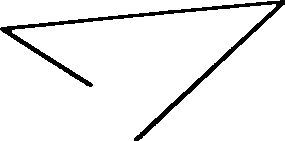
\includegraphics[width=0.75\textwidth]{figures/quad1.png}
	\end{subfigure}
	\begin{subfigure}{0.5\textwidth}
		\centering
		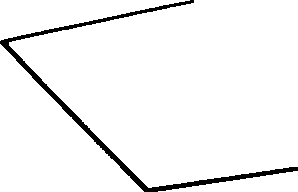
\includegraphics[width=0.75\textwidth]{figures/quad2.png}
	\end{subfigure}
	\caption{Example for different quads}
	\label{fig:exampleQuads}
\end{figure}

%-----------------------------------------------------------------------------------------------
\section{RQIM}
%-----------------------------------------------------------------------------------------------
